\section{Development and testing}

\subsection{Hardware assembly}

\subsection{Programming the hardware}

\subsection{Range tests}

One of the most important tests to carry out prior to deployment in the field
was testing the range of the devices.

In this experiment I took four challenger RP2040s to The Downs, a large public
park in Bristol. Here I tested four different antenna configurations to compare
how well the signal travelled across an increasing distance. Signal strength can
be measured using the received signal strength index (RSSI) while quality of the
signal was measured using the signal-to-noise ratio (SNR). 

For the test, two challengers were programmed as transmitters, sending an
example data packet similar to the data that would eventually be used at the
farm. One of the transmitters used the simple PCB antenna
(Figure~\ref{fig:pcb-antenna}) while the other used a higher range whip style
antenna (Figure~\ref{fig:good-antenna}). Then I programmed two challengers as
receivers, again one had a low range antenna and the other a long range one.

This meant that four different antenna configurations could be tested
concurrently, as the receivers could pick up the signal from each transmitter.
An estimate of their relative performance before testing is shown below:

\begin{enumerate}
    \item Whip antenna to whip antenna (Likely best result)
    \item PCB antenna to whip antenna
    \item Whip antenna to PCB antenna
    \item PCB antenna to PCB antenna (Likely poorest result)
\end{enumerate}

The reason PCB transmitter to whip receiver will likely outperform the whip to
PCB configuration is that generally it is more important that the receiver has
better "hearing" capabilities than the transmitter can "shout".

Nine different distances were from transmitter to receiver were tested, in 200m
increments starting from 0m as a baseline to a distance of 1600m
(Figure~\ref{fig:range-test-markers}). An important aspect in getting a
successful LoRa connection is whether there is line of sight between the
transmitter and receiver. Figure~\ref{fig:range-test-elevation} shows the
elevation profile of the test area, with the initial large dip being an
inaccuracy from google earth's topology data as the 0m point is near a cliff
edge. The lowest elevation point is at the starting point at around 83m above
sea level, while the highest point was at the 1km mark at around 94m making an
elevation range of 11m. My hypothesis was that signal would likely drop off or
stop entirely beyond this point as points beyond 1000m would be below the hill
line. This would effectively mean that the receivers would be in a signal shadow
point where the transmission waves would not be able to reach them. The only
possibility for signal to reach this area would be from reflections either from
nearby buildings or topology. However the effects of reflections are virtually
impossible to account for in the real world and therefore no accurate
predictions could be made.

\begin{figure}[H]
    \centering
    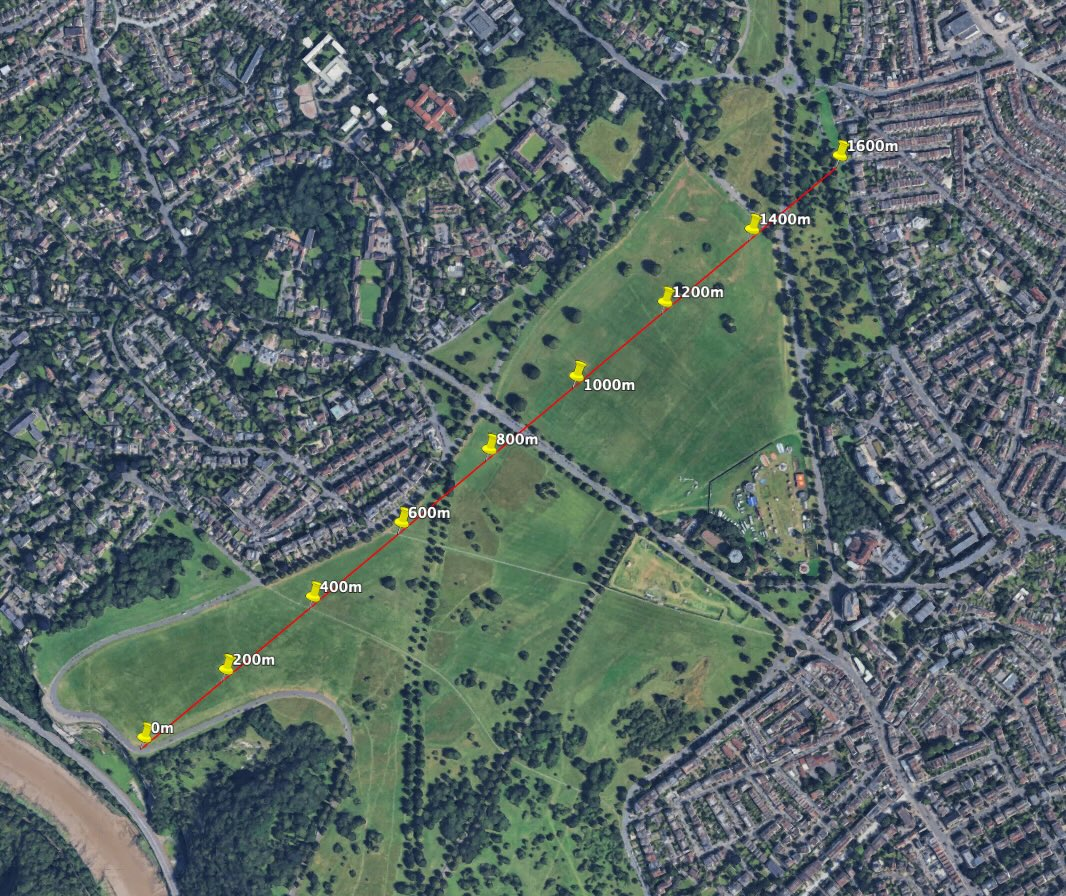
\includegraphics[width=0.8\textwidth]{contents/23-hw-development/23-fig/range-test-markers.jpg}
    \caption{Google earth image of data collection points}
    \label{fig:range-test-markers}
\end{figure}


\begin{figure}[H]
    \centering
    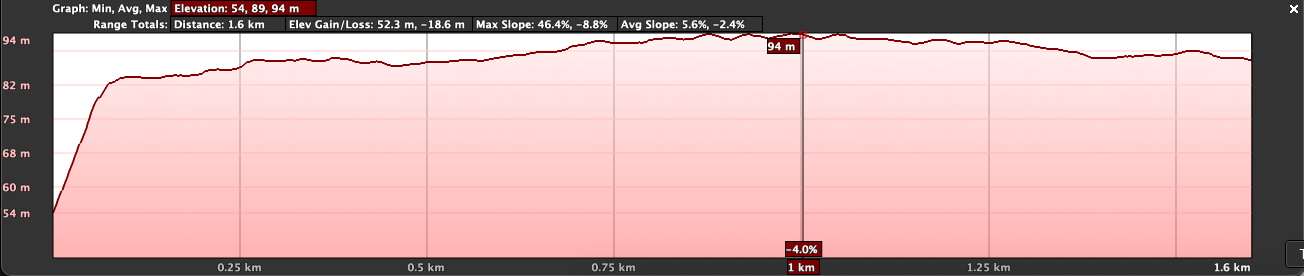
\includegraphics[width=1\textwidth]{contents/23-hw-development/23-fig/range-test-elevation-profile.jpg}
    \caption{Elevation profile of test area (ignore large dip at start)}
    \label{fig:range-test-elevation}
\end{figure}


